\documentclass[a4paper]{jpconf}
\usepackage{graphicx}
\usepackage{draftwatermark}
\usepackage[margin=0.8in]{geometry}
\usepackage{lmodern}% http://ctan.org/pkg/lm
\usepackage{listings}
\usepackage[utf8]{inputenc}
\usepackage[toc,page]{appendix}
%\usepackage{wrapfig}
%\usepackage{float}
\usepackage{hyperref}
\usepackage{listings}
\usepackage{citesort}
\usepackage{changepage}
\usepackage{caption}
\usepackage{color}
\usepackage{courier}
\usepackage{subcaption}
\usepackage{hyperref}\begin{document}
\title{Profiling ATLAS Kit Validation on \newline Intel Haswell-EP processors}

\author{M Guerri$^1$, D Giordano$^1$, C Cordeiro$^1$}
\address{$^1$ CERN}
\ead{marco.guerri@cern.ch}
\SetWatermarkText{DRAFT}
\definecolor{lightblue}{gray}{0.95}

\lstset{
    language=Python,
    basicstyle=\sffamily,
    tabsize=2,
    backgroundcolor=\color{lightblue},
    captionpos=b,
    %numbers=left,
    columns=1,
    keepspaces=true,
    showstringspaces=false,
    stepnumber=1,
    numberstyle=\scriptsize,
    numbersep=5pt,
    frame=lines,
    escapeinside={£}{£},
    breaklines=true,
    keywordstyle=\color[rgb]{0,0,1},
    commentstyle=\color[rgb]{0.133,0.545,0.133},
    stringstyle=\color[rgb]{1,0,0}
}

\begin{abstract}
With the increasing adoption of cloud resources, public and private, to support
the demands in terms of computing capacity of the WLCG, the HEP community has begun
studying several benchmarking applications aimed at continuously assessing the
performance of virtual machines procured from commercial providers.
In order to characterise the behaviour of these benchmarks, in-depth
profiling activities have been carried out. In this document we outline
our experience in profiling one specific application, ATLAS Kit Validation,
in an attempt to explain an unexpected distribution of the performance samples
obtained on systems based on Intel Haswell-EP processors.
\end{abstract}


\section{Introduction}
Nowadays the majority of the experiments' workloads running on the WLCG are simulation 
jobs, where most of the computing time is spent in CPU-bound activities. For this 
reason the adoption of fast benchmarks representative of these workloads 
can be beneficial for monitoring and resource allocation purposes,
by providing real-time information on the performance delivered by virtual 
machines in the cloud or job slots in a grid site.
%For instance a prompt benchmarking can  act as a prediction mechanism for the 
%execution of the LHC experiments' workloads, allowing for a fast and reliable 
%triage of suitable resources in a much shorter time period than standard jobs.
A number of fast benchmarks is being studied by the HEP community. Within the 
HEPiX Benchmarking Working Group~\cite{HEPiX:2014:HEPiX}, two fast benchmarks are 
in particular under deep investigation: Dirac Benchmark 2012 (DB12)~\cite{CERN:2016:DB12} 
and ATLAS Kit Validation (KV)~\cite{KV}.

\section{KV Benchmark}
KV is the toolkit adopted by the ATLAS collaboration for the
validation of their software installation in grid sites. The tests include, among
others, the GEANT4~\cite{GEANT4} simulation of the ATLAS detector, which
has been re-purposed to benchmark compute resources against CPU-bound 
workloads. The KV benchmark simulates $n$ independent events consisting of a single muon particle 
propagating through the ATLAS detector. The CPU time needed to elaborate each event 
is recorded and the average over the $n$ events is computed as the final benchmark result.
By excluding the first event in the sequence from the final average, spurious effects such as the 
overhead coming from the initialisation of the software libraries and the configuration 
of the simulation parameters (detector geometry, list of particles, properties of 
the materials) are disregarded from the measurement.

The KV benchmark is single threaded as most of the LHC experiments'
software applications. In order to fully utilize compute resources and reproduce
the worst case load scenario, where all compute slots are running jobs and
CPU idle time is minimised, the benchmark is configured to run,
by default, in parallel with as many threads as the number of logical cores 
provided by the server and the benchmark result is calculated as the arithmetic 
average over all threads.

In the past few years the KV benchmark has been used to assess the performance of
resources provided by commercial cloud providers and grid site. The results 
have been compared with the average CPU time required to simulate ATLAS events, 
as reported by the experiment's job monitoring framework. Details about this activity 
and the correlation among benchmark results and job duration are reported 
in~\cite{bmk}.


\section{Investigating KV results}
One of the several environments that was benchmarked using KV consisted of
 240 Haswell-EP hypervisors providing compute
resources as VMs dedicated to the CERN Tier-0 batch system. The servers were
fitted with two 8-core Intel Xeon E5-2630v3 processors, with a total number  
of 32 threads per server with simultaneous multithreading enabled, and 64~GiB    
of DDR4 RAM in fully balanced configuration, with each memory channel populated with
the same number of DIMMs of equal capacity. All the hypervisors were configured 
to host 2 VMs providing 16 virtual processing units each, with pairs of VMs 
confined to separate NUMA domains. KV was executed with 16 parallel processes 
on each VM, resulting in the full utilisation of the hardware threads provided
by the machine, and the final aggregated result was obtained as the average over 
the 16 simulation times. The samples collected from the VMs under test resulted in a dual-mode guassian distribution, with a 2\% difference between the 
mean of the two modes as shown in Figure~\ref{dual-mode-gaussian}.


\begin{figure}[ht]
\begin{center}
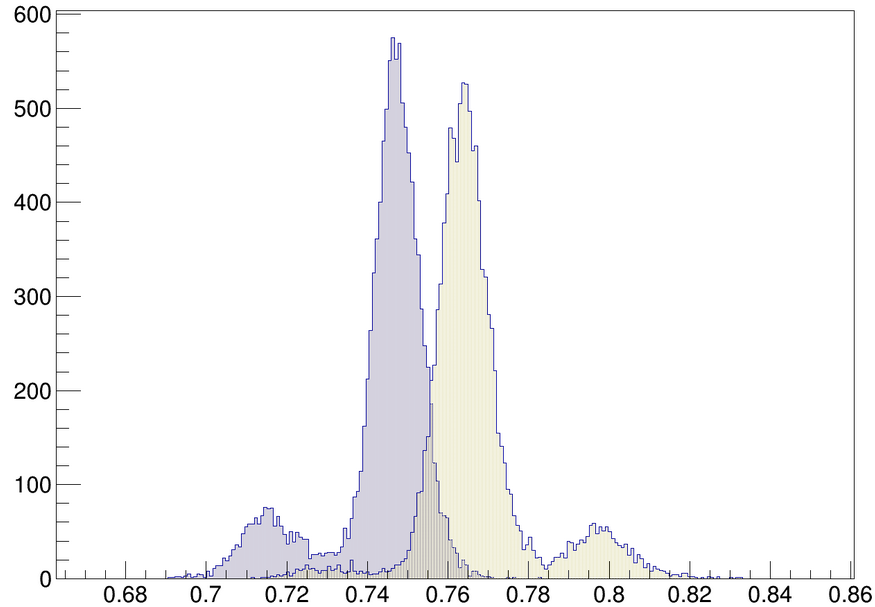
\includegraphics[width=0.5\textwidth]{images/dual-mode-gaussian.png}
\end{center}
\caption{\label{dual-mode-gaussian} Distribution of the average KV execution speed [sec/evt] on  VMs with 16 virtual CPUs. }
\end{figure}




%\section{Bare metal results}
In order to ease the performance analysis, the virtualisation layer was
temporarily removed and Simultaneous Multithreading disabled, running KV on 
the bare-metal server while setting scheduling affinity sequentially to each physical
core. The results shown
in Figure~\ref{kv-runtime} highlighted a 12\% difference in the average simulation
time when binding KV to core 8, the first core of the second processor, i.e. CPU1.

\begin{figure}[b]
\begin{center}
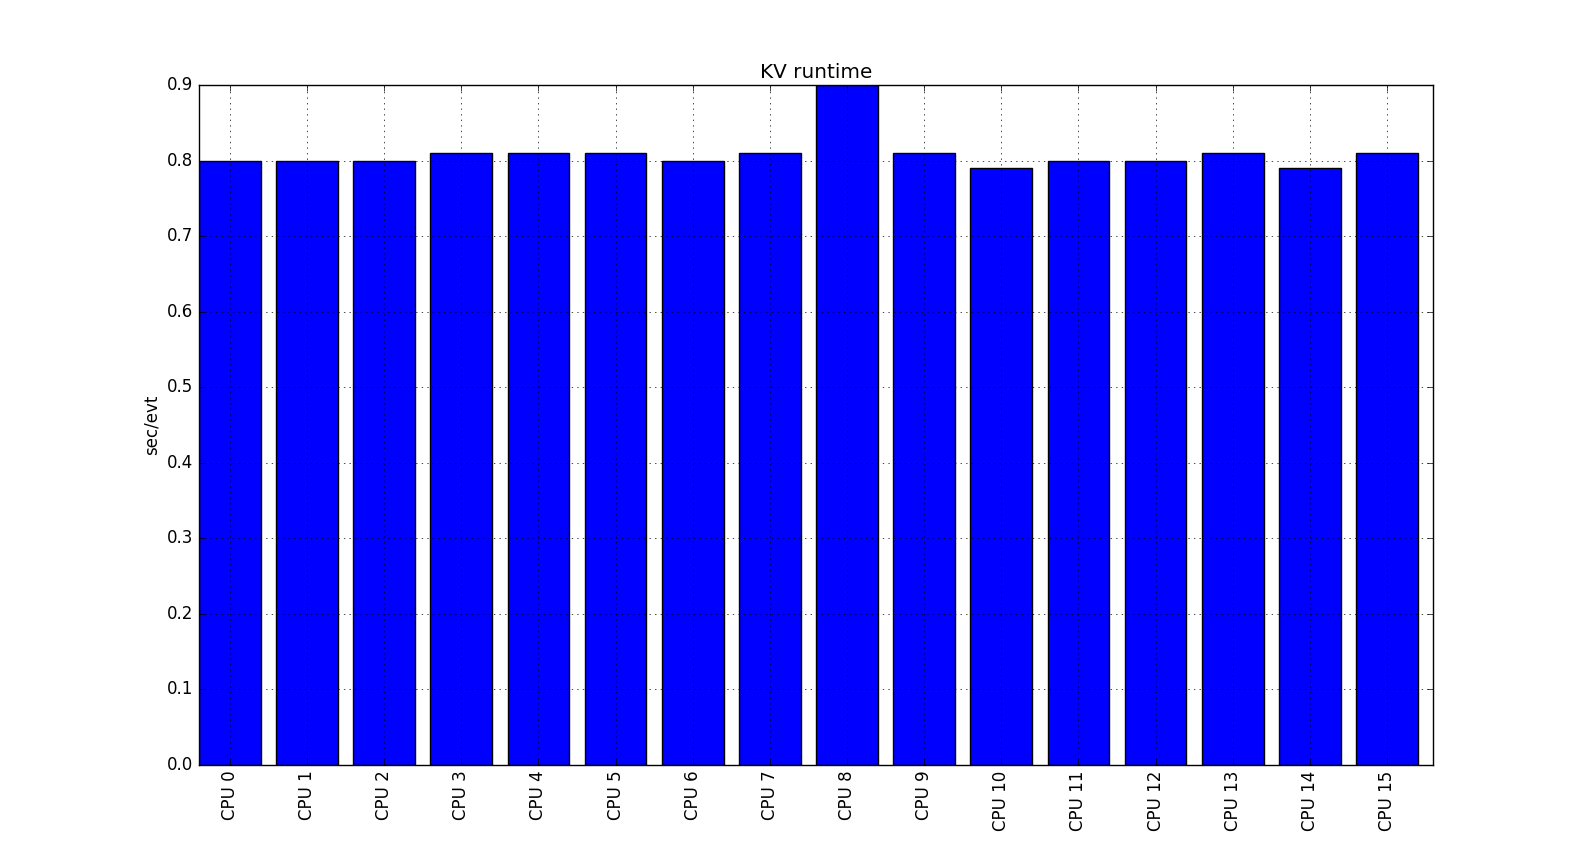
\includegraphics[scale=0.3]{images/kv_runtime.png}
\end{center}
\caption{\label{kv-runtime} Bare-metal KV performance (sec/evt) on each physical core. }
\end{figure}
Further tests confirmed the same behaviour also with Simultaneous Multithreading 
on, with slower performance on thread 8 and 24, both belonging to the first core of 
CPU1. Single thread runs in a virtualised environment showed a 16\%
increase in the final average simulation time when running on virtual processors
corresponding to hardware threads 8 and 24, confirming the 2\%
spread that stood out from the statistical distribution after averaging the results
over all 8 virtual processors within each VM. 


\section{Profiling single events}
A deeper dive in the logs showed that all the events required more time to be 
simulated on core 8. In particular, event 73 was identified as the one
requiring the longest simulation time: ~34 seconds on core 8 against ~29 seconds
on any other core, making it a good candidate for an in-depth analysis. Profiling 
a single event required a way to attach \textit{perf} to KV only during the time frame
where one specific simulation was being executed. The solution adopted consisted
in a Python script which would monitor KV log files via \textit{pyinotify} to detect
the beginning of event 73. The script would attach \textit{perf} to KV until the
detection of the end of event. One essential requirement for this to work correctly
was to disable all the buffering carried out at any layer of the stack before
data actually reaching the storage device. KV writes log files via Python code,
therefore the following points had be taken into consideration:
%\begin{lstlisting}[caption=Simulation of event 73 on core 8, basicstyle=\scriptsize]
%*  Memory snooper called at end of event with VMEM: 1443232kB
%G4SimTimer           INFO        Event nr. 73 took 34.58 s. New average 0.985 +- 0.4806
%AtRndmGenSvc         INFO  Stream =  SINGLE, Seed1 =  93448506, Seed2 = 144728191
%AthenaEventLoopMgr   INFO  done processing event #72, run #1 73 events processed so far
%AthenaEventLoopMgr   INFO  start processing event #73, run #1 73 events processed so far
%G4AtlasAlg           INFO ++++++++++++  G4AtlasAlg execute  ++++++++++++
%\end{lstlisting}

%\begin{lstlisting}[caption=Simulation of event 73 on core 0, basicstyle=\scriptsize]
%*  Memory snooper called at end of event with VMEM: 1443252kB
%G4SimTimer           INFO        Event nr. 73 took 29.68 s. New average 0.8681 +- 0.4133
%AtRndmGenSvc         INFO  Stream =  SINGLE, Seed1 =  93448506, Seed2 = 144728191
%AthenaEventLoopMgr   INFO  done processing event #72, run #1 73 events processed so far 
%AthenaEventLoopMgr   INFO  start processing event #73, run #1 73 events processed so far
%G4AtlasAlg           INFO ++++++++++++  G4AtlasAlg execute  ++++++++++++
%\end{lstlisting}

\begin{itemize}
\item A call to \textit{open} function in Python, results in the invocation
of libc \textit{fopen}. Python can modify libc buffering behaviour via libc 
function \textit{setvbuf} if \textit{buffering} parameter is specified, 
otherwise the default libc buffering is used. Without control over the Python
source code, it was not possible to modify buffering options.
\item Environment variable \textit{PYTHONUNBUFFERED} can be used to turn off
buffering of \textit{stdin, stdout, stderr}.
\end{itemize}
The best solution found to implement unbuffered I/O to log files was to set 
\textit{PYTHONUNBUFFERED=1} and pipe logs printed by KV on standard output to
\textit{tee}, which would eventually write to an additional log file setting 
\textit{\_IONBF} on all file descriptors via \textit{setvbuf}.
\textit{unbuffer} command was also used to disable buffering between the two
ends of the pipe. 
\\
The profile of the execution was obtained with \textit{perf record} . 
Results for core 8 
and core 0 are shown respectively in figure ~\ref{event-73-processor8} and 
figure ~\ref{event-73-processor0} (limiting the output to the functions that
account for more than 1\% of the runtime). 

\begin{figure}[h]
\begin{center}
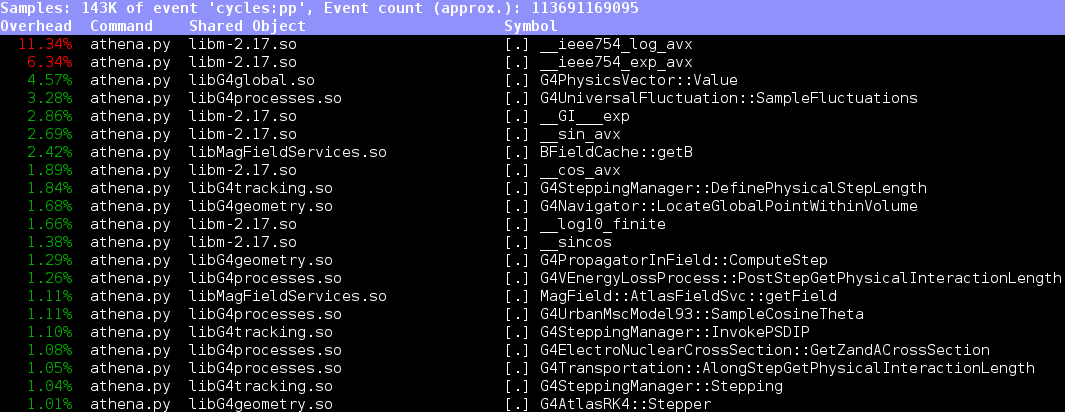
\includegraphics[scale=0.45]{images/Event73_Processor8.png}
\end{center}
\caption{\label{event-73-processor8} Recording of event 73 on core 8}
\end{figure}

\begin{figure}[h]
\begin{center}
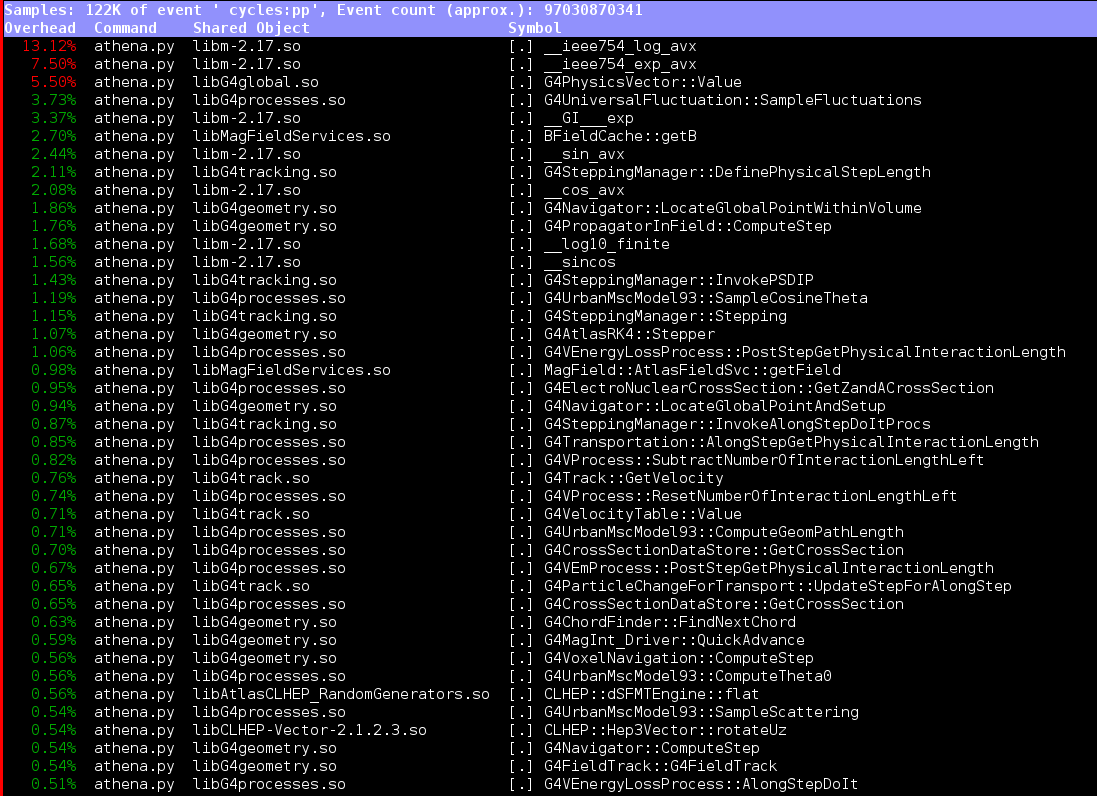
\includegraphics[scale=0.45]{images/Event73_Processor0.png}
\end{center}
\caption{\label{event-73-processor0} Recording of event 73 on core 0}
\end{figure}

Excluding the higher number of events
(unhalted core cycles) on core 8, which was expected due to the longer runtime,
it was not possible to identify any major difference between the two runs, which
were showing the same functions coming mostly from \textit{libm} and \textit{Gean4} 
libraries. These results were then elaborated into a list of the top contributors 
to the additional clock cycles required when running on core 8 as shown 
in table ~\ref{major-contributors}.

\begin{table}
\begin{center}
\begin{tabular}{ | l | l |}
    \hline
	\_\_sin\_avx & 4.14\% \\
	\hline
	G4VEnergyLossProcess::PostStepGetPhysicalInteractionLength & 2.40\% \\
    \hline
 	FADS::FadsSteppingAction::UserSteppingAction & 2.26\% \\
    \hline
	G4Transportation::AlongStepGetPhysicalInteractionLength & 2.18\% \\
    \hline
	G4ParticleChangeForTransport::UpdateStepForAlongStep & 2.07\% \\
    \hline
	MagField::AtlasFieldSvc::getField & 1.86\% \\
    \hline
	G4ElectroNuclearCrossSection::GetZandACrossSection	& 1.85\% \\
	\hline
	G4Tubs::DistanceToOut & 1.62\% \\
	\hline
	G4CrossSectionDataStore::GetCrossSection & 1.59\% \\
	\hline
	\_\_log10\_finite &	1.53\% \\
	\hline
\end{tabular}
\end{center}
\caption{Major contributors to the additional runtime on core 8 (percentage
of the additional clock cycles) }
\label{major-contributors}
\end{table}

\section{Profiling the major contributors}
After having obtained the list in table ~\ref{major-contributors}, the 
top contributors to the additional runtime were profiled to obtain
a detailed breakdown of the weight of each assembly instruction in terms of 
clock cycles. The recordings of \textit{\_\_sin\_avx}, 
\textit{PostStepGetPhysicalInteractionLength}, \textit{UserSteppingAction},
\textit{UpdateStepForAlongStep}, \textit{GetZandACrossSection},
\textit{DistanceToOut}, \textit{GetCrossSection} and \textit{\_\_log10\_finite}
 are reported in Appendix  
~\ref{appending:function-recording}. The results highlighted an interesting 
pattern on most of the major contributors:  it appeared that an unexpectedly 
large number of cycles was attributed to the initial instructions of each function.
Most of these instructions, despite sometimes accessing memory 
(e.g. push on the stack), could not justify such a high cost: in some cases a 
\textit{mov} of a literal value to a register was taking up 8\% of the whole 
execution time of that specific function. Such behavior was common to all cores,
but if these functions were responsible for most of the additional execution time,
then probably the reason had to be related to this peculiar profile. A first hypothesis
pointed in the direction of instruction cache misses as the reason behind
the large number of cycles spent on the initial instructions.
ATLAS Kit Validation seemed a good candidate for a large number of  such events,
with its large code segment consisting of tens of shared libraries. Even though
this hypothesis could not explain the slower performance when running on core 8,
an attempt was made to validate it.
 

\section{Synthetic benchmark to generate instruction cache miss}
A synthetic benchmark aimed at causing a large number of instruction cache 
misses was automatically generated using a \href{https://gitlab.cern.ch/snippets/216}{Python script}. The resulting C code was compiled
under CentOS 7 with gcc 4.8.5 and \textit{-O0}. The benchmark consists of a large
number of dummy functions which are called randomly at runtime, generating
repeated instruction cache misses in L1i and L2. Interestingly, the results
highlighted the same performance asymmetry observed with ATLAS Kit Validation,
with a 20\% increase in runtime on core 8 with respect to the other cores.
This effect could only be observed on the following systems:
\begin{itemize}
    \item Haswell-EP
    \item Haswell-EX (quad-socket, with a single core on two different sockets affected)
    \item Broadwell-EP
\end{itemize}
All the attempts to reproduce a similar performance asymmetry on Sandy Bridge
and Ivy Bridge failed.
%\begin{figure}[h]
%\begin{center}
%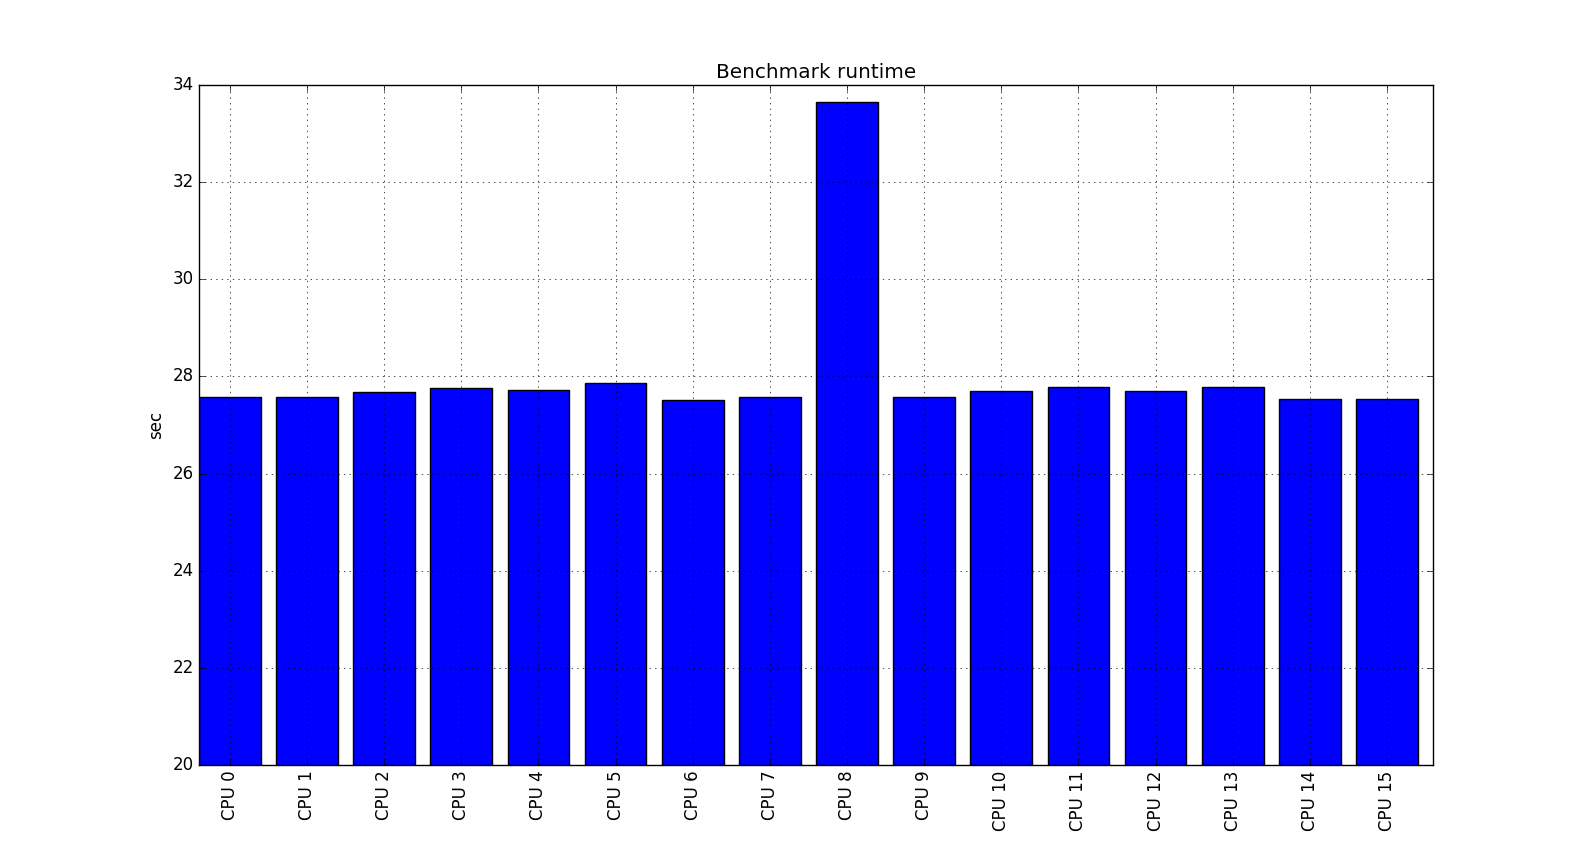
\includegraphics[scale=0.45]{images/syn-bench-a.png}
%\end{center}
%\caption{\label{syn-bench-a} Runtime of the synthetic benchmark (random calls)}
%\end{figure}
Further investigations succeeded in generating
workloads with similar relative number of L1i and L2 instruction cache misses
on Haswell and Broadwell, but without any discrepancy in execution time, 
disproving the initial hypothesis and making it necessary to seek for an 
alternative explanation.

\section{Additional benchmark with customizable code segment size}
\label{section:benchmark-itlb}
\href{https://gitlab.cern.ch/snippets/217}{A second synthetic benchmark} 
was written in order to verify the existence of a 
correlation between the size of the code segment and the performance 
asymmetry. This benchmark is also aimed at generating instruction cache misses,
but within a code segment whose size can be controlled via a command line 
argument. The code makes use of a large switch statement that dispatches
opcodes randomly generated. This operation is performed in loop: 
by feeding the switch with $opcode\pmod n$, the number of case 
branches effectively used is limited to $n$. The higher $n$, the larger the
number of case branches that can be reached. By ``sampling'' the 
maximum and minimum values of \textit{rip} register, a reliable estimate of the 
size of the hot portion of the code segment can be obtained. The
benchmark accepts $n$ as command line argument and prints a tuple consisting of
three values: \textit{(size code segment, runtime without initialization, n)}.
The graph in figure ~\ref{fig:runtime-difference} shows the difference in runtime 
between core 8 and core 0 with respect to the size of the code segment. Excluding a
negligible number of outliers, the samples collected clearly highlighted a performance 
degradation beyond approximately 512KiB, with core 8 running up to 4 seconds slower
(9.4\%) in the 3MB area. 512KiB is an interesting number, as it 
corresponds to the space addressable with 128 iTLB entries using 4KiB pages. 
Haswell and Broadwell architectures use an iTLB with exactly 128 entries. 
Beyond 512KiB, a heavily non linear execution flow starts generating an increasingly 
large number of iTLB misses. Although the reason is not clear, this test pointed
in the direction of a different behavior of the front-end of the pipeline 
in handling such events.
\\
The test was repeated by making use of the huge pages support of the operating
system (2MiB). The following commands were used to compile and execute the benchmark
with a code segment size of 3 MiB.

\begin{lstlisting}
sysctl vm.nr_hugepages=500
gcc benchmark.c -o benchmark -O0 -B/usr/share/libhugetlbfs -Wl,--hugetlbfs-align
hugectl --text ./switch_slowdown_v2 32768
\end{lstlisting}
With 2MiB pages, no performance difference was observed between core 8 and the 
other cores on the system.

\begin{figure}[h]
\begin{center}
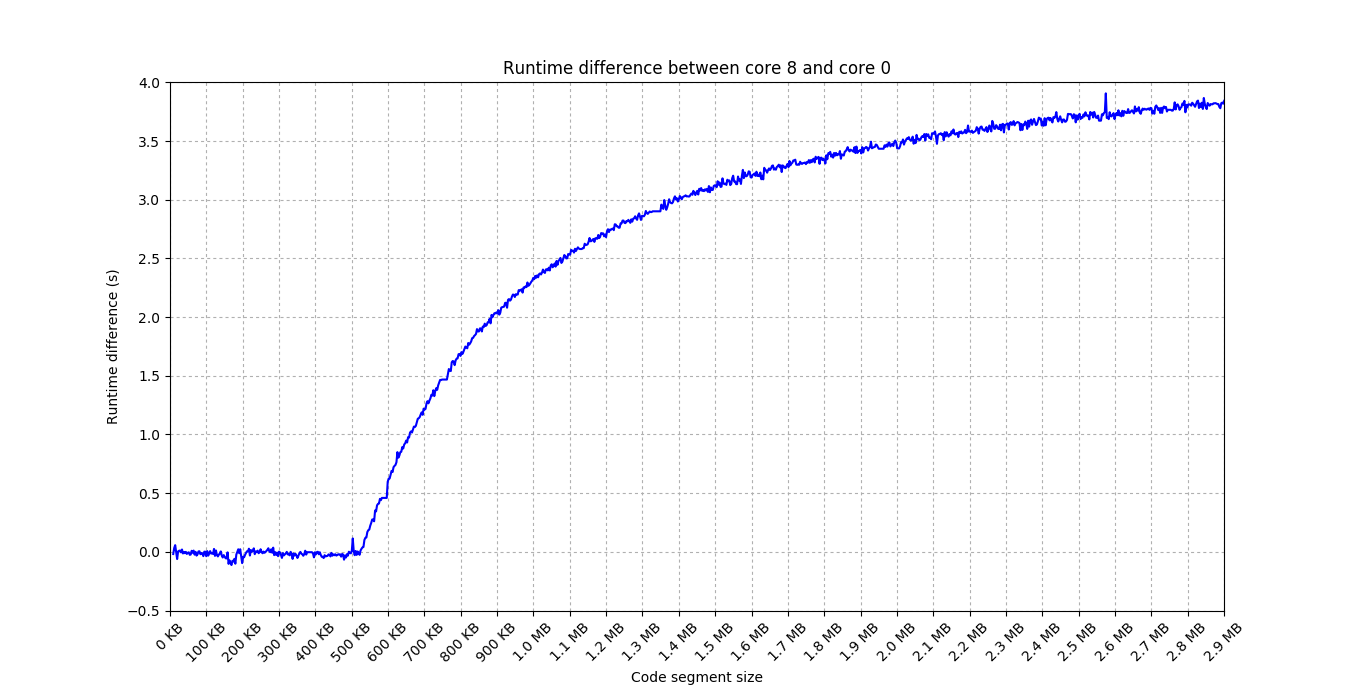
\includegraphics[scale=0.45]{images/runtime_difference.png}
\end{center}
\caption{\label{fig:runtime-difference} Runtime difference between core 8 and core 0}
\end{figure}

\section{Hypothesis disproved so far}
The following hypothesis have been taken into account so far, without however
leading to a satisfactory explanation:

\begin{itemize}
\item \textit{ksoftirq is using more clock cycles on core 8, therefore there 
appears to be more interrupt activity (at least top half) on this specific core.}
\\
The additional number of cycles spent in \textit{\_\_do\_softirq} does not justify 
the slowdown observed. The profiles of the benchmark described in section
\ref{section:benchmark-itlb} with $n = 32000$ show that \textit{\_\_do\_softirq}
and \textit{do\_softirq} are responsible respectively for 0.08\% and 0.05\% of the 
additional clock cycles on core 8. The higher number of cycles spent in softirq
seems to be a consequence rather than a cause. In the Linux kernel the top half 
of the timer interrupt is implemented with a softirq, so it makes sense to have 
a higher number softirqs running if the runtime of the benchmark is itself longer
(1ms jiffie).
\end{itemize}


\begin{appendices}

\section{Function recordings}
\label{appending:function-recording}
\begin{figure}[H]
\begin{center}
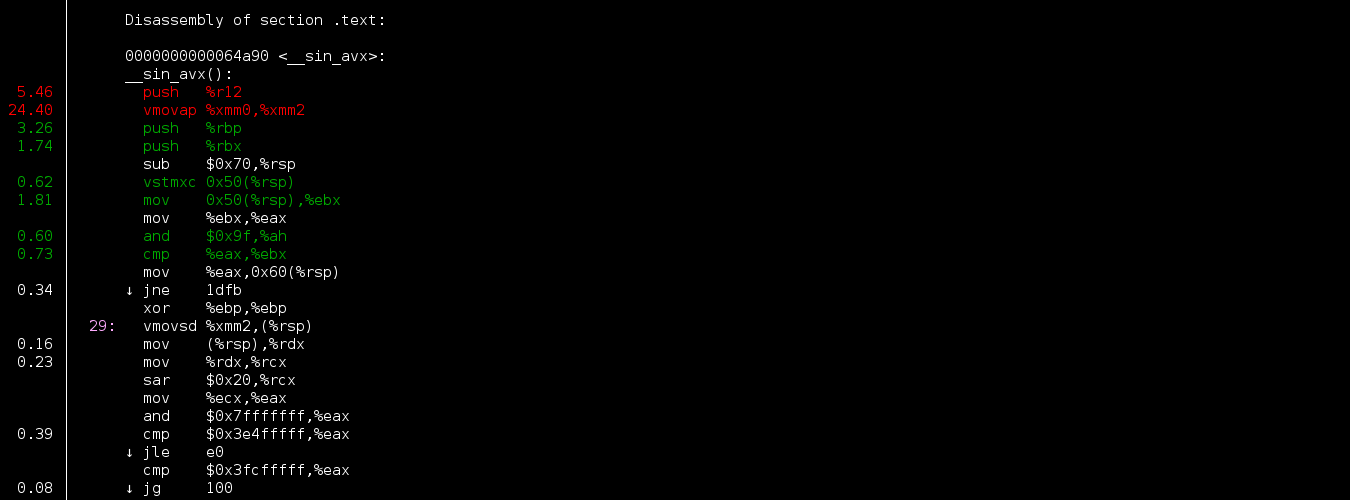
\includegraphics[scale=0.33]{images/sin_P8.png}
\caption{\_\_sin\_avx}
\end{center}
\end{figure}

\begin{figure}[H]
\begin{center}
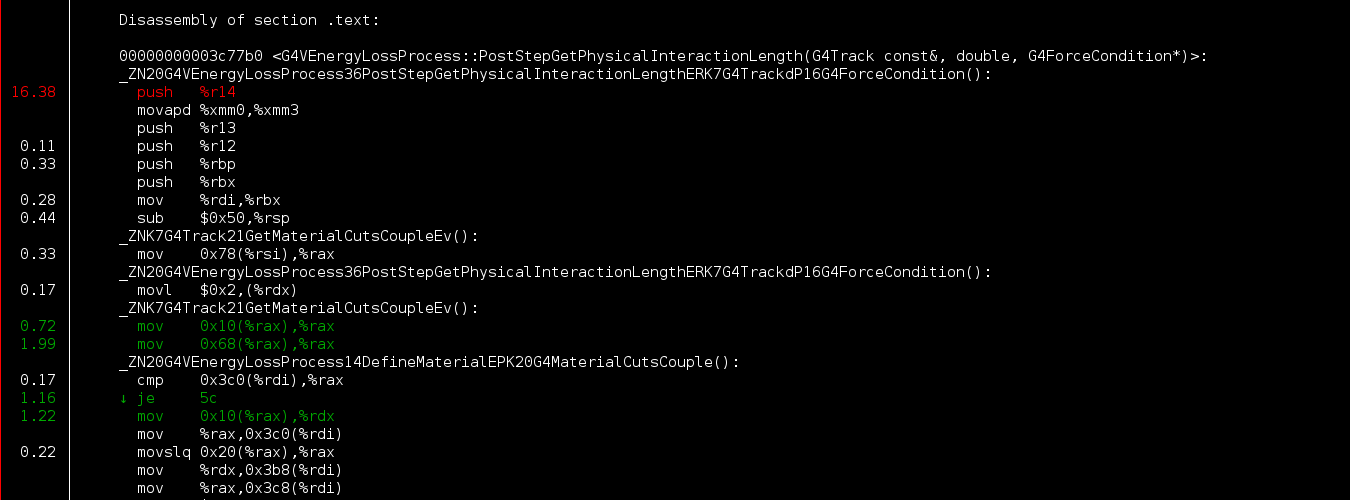
\includegraphics[scale=0.33]{images/Post_step_P8.png}
\caption{PostStepGetPhysicalInteractionLength}
\end{center}
\end{figure}

\begin{figure}[H]
\begin{center}
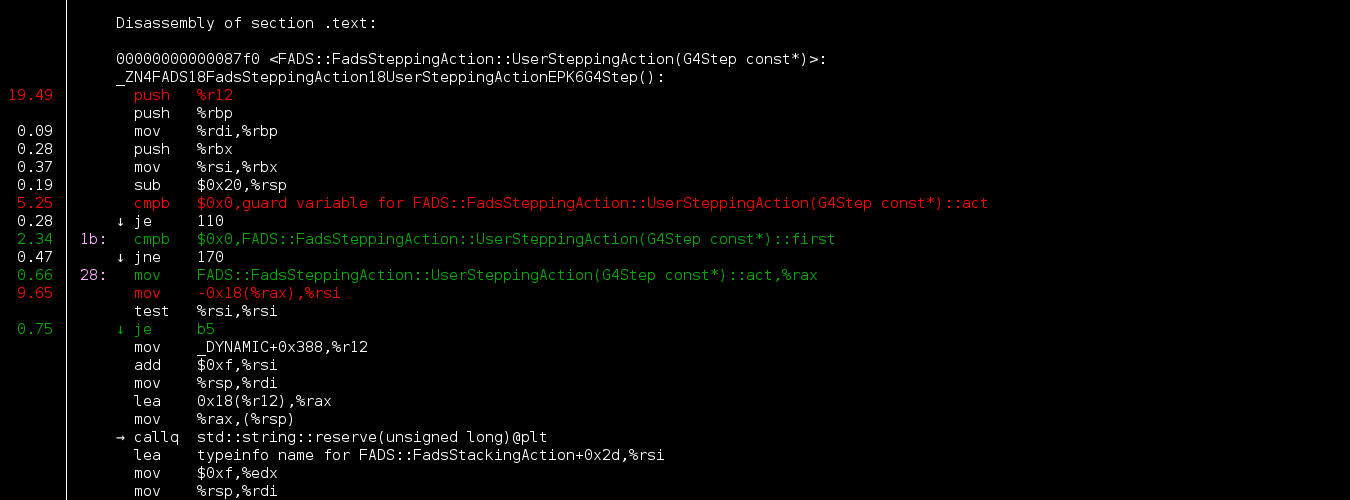
\includegraphics[scale=0.33]{images/UserStepping_P8.png}
\caption{UserSteppingAction}
\end{center}
\end{figure}

\begin{figure}[H]
\begin{center}
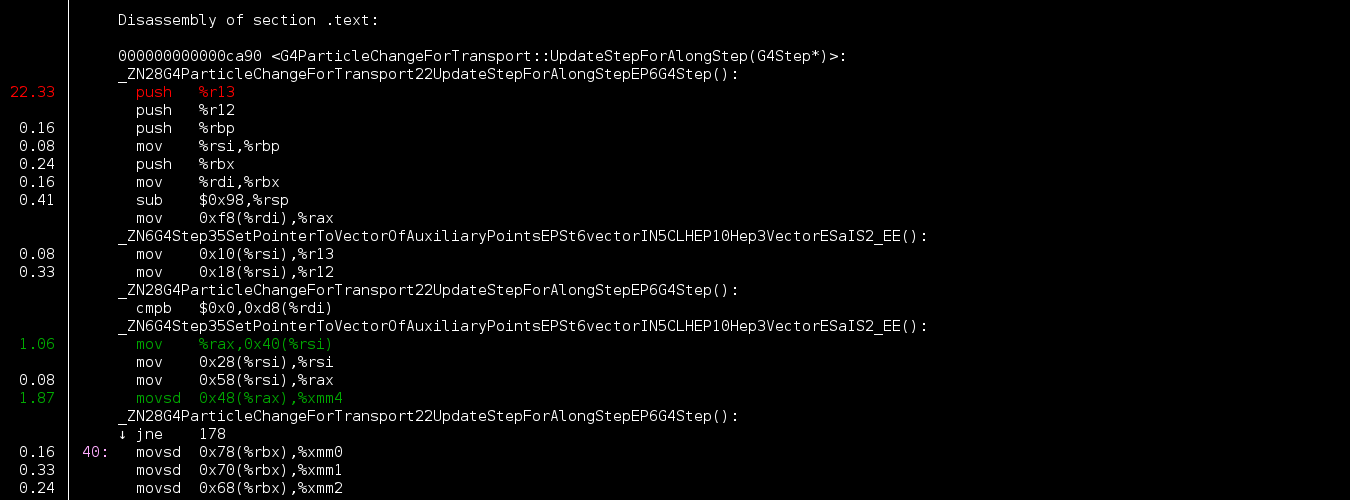
\includegraphics[scale=0.33]{images/UpdateForAlongStep_P8.png}
\caption{UpdateStepForAlongStep}
\end{center}
\end{figure}

\begin{figure}[H]
\begin{center}
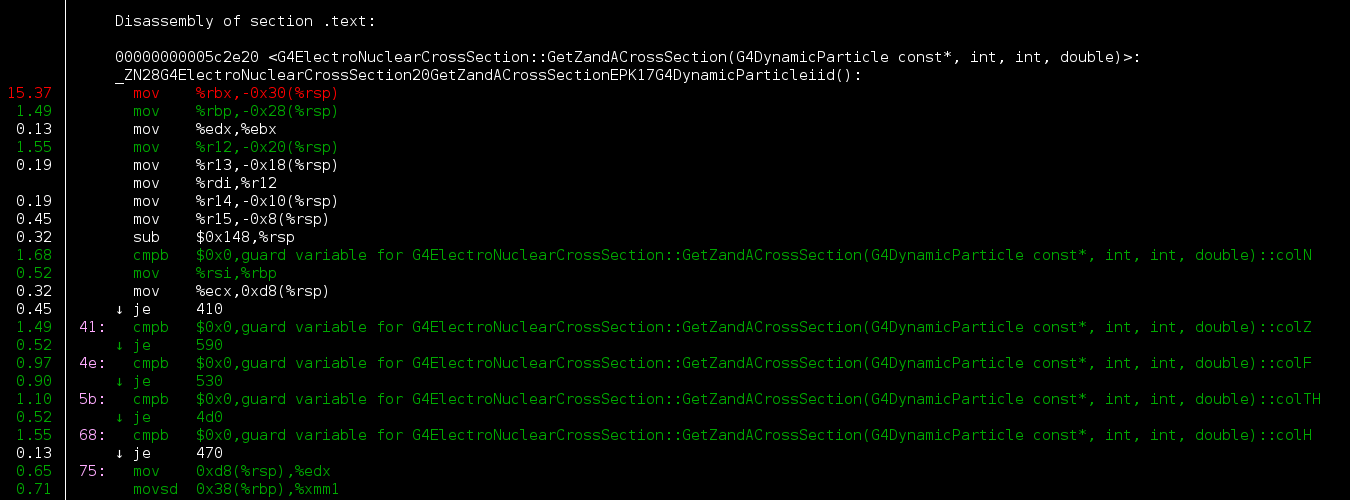
\includegraphics[scale=0.33]{images/GetZandACrossSection_P8.png}
\caption{GetZandACrossSection}
\end{center}
\end{figure}

\begin{figure}[H]
\begin{center}
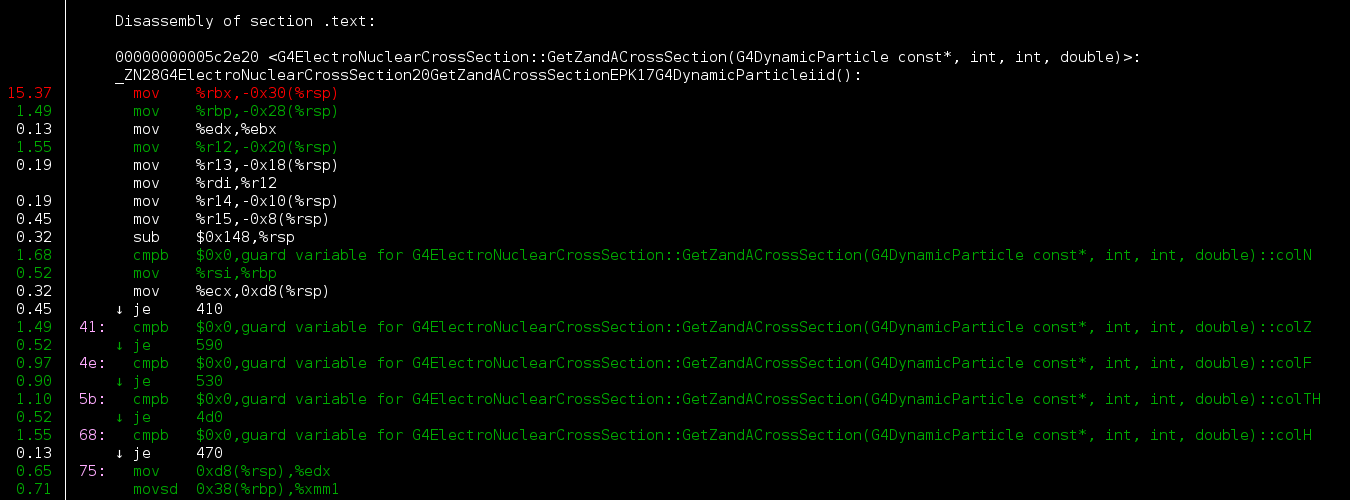
\includegraphics[scale=0.33]{images/GetZandACrossSection_P8.png}
\caption{GetZandACrossSection}
\end{center}
\end{figure}

\begin{figure}[H]
\begin{center}
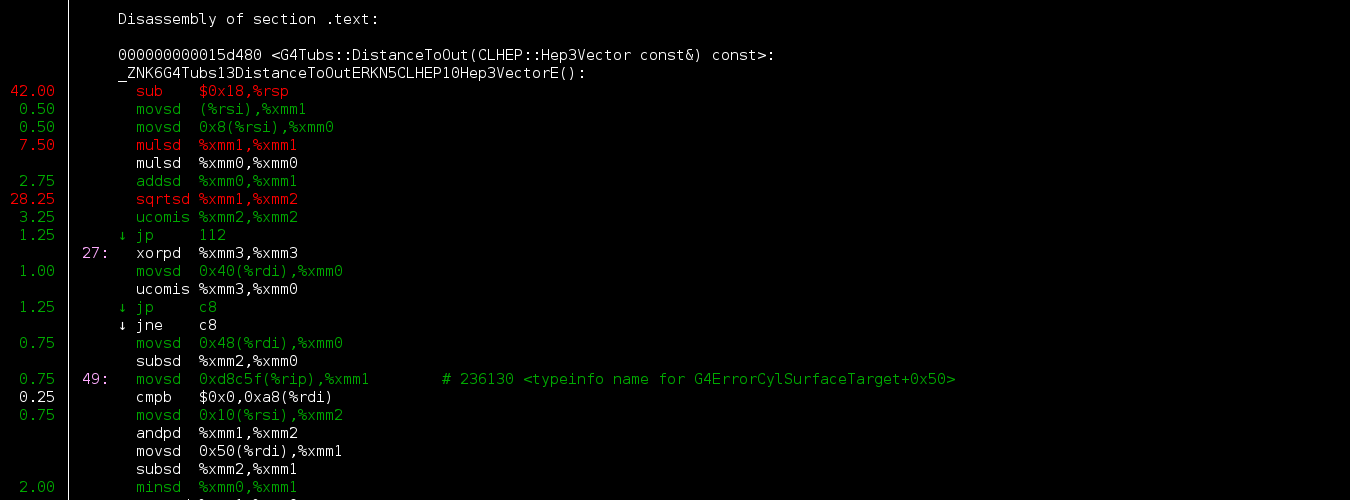
\includegraphics[scale=0.33]{images/DistanceToOut_P8.png}
\caption{DistanceToOut}
\end{center}
\end{figure}

\begin{figure}[H]
\begin{center}
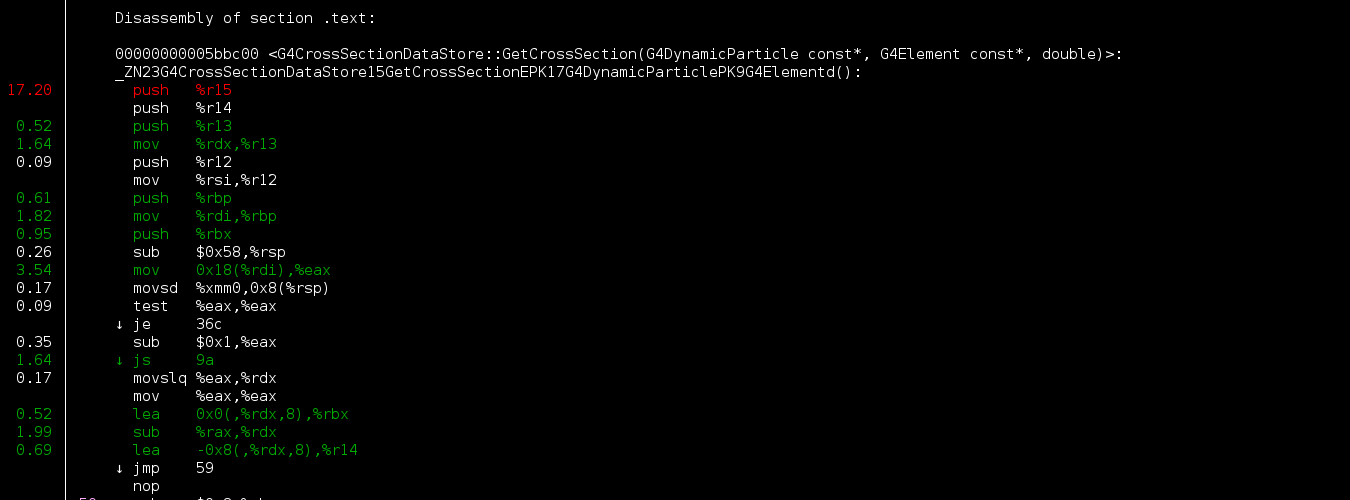
\includegraphics[scale=0.33]{images/GetCrossSection_P8.png}
\caption{GetCrossSection}
\end{center}
\end{figure}

\begin{figure}[H]
\begin{center}
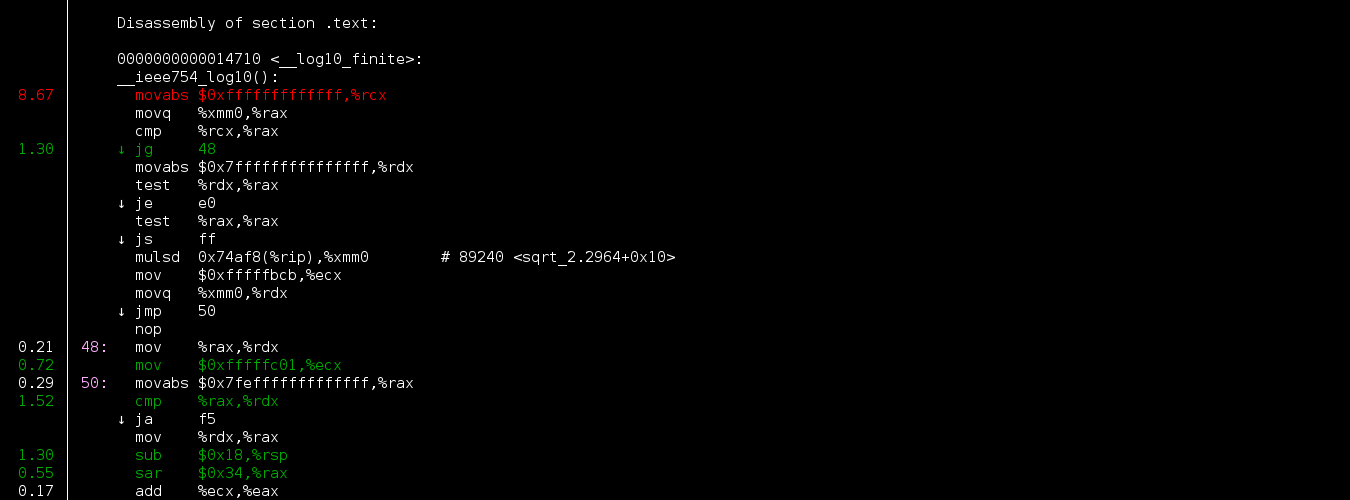
\includegraphics[scale=0.33]{images/__log10_finite_P8.png}
\caption{\_\_log10\_finite}
\end{center}
\end{figure}


\end{appendices}
%\section*{References}
%\bibliography{iopart-num}
%\bibliographystyle{unsrt}
\end{document}
